\documentclass[a4paper,12pt]{report}
\usepackage[top=1in,bottom=1in,left=1in,right=1in]{geometry} 
\usepackage{amsfonts, amsmath, amssymb}
\usepackage{graphicx}
\usepackage{times}
\usepackage{float}
\usepackage[section]{placeins}
\usepackage[skip = 8pt,tableposition=top, figureposition=bottom]{caption}
\usepackage{hyperref}
\usepackage[section]{placeins}
\usepackage{setspace}
\usepackage{acro}
\makeatletter
\def\@makechapterhead#1{%
  %\vspace*{50pt}%
  {  \MakeUppercase{\ifnum \c@secnumdepth >\m@ne
        \fontsize{16pt}{1}\bfseries \@chapapp \space \thechapter\vspace{5pt}\\
    \fi
    \interlinepenalty\@M
     \bfseries #1}\par\nobreak
    %\vskip 0pt
  }}
  \makeatletter
% Redefine the \chapter* header macro to remove vertical space
\def\@makeschapterhead#1{%
  %\vspace*{50\p@}% Remove the vertical space
  {\newpage \parindent \z@ \raggedright
    \normalfont
    \interlinepenalty\@M
    \center \fontsize{16pt}{1} \bfseries \MakeUppercase{#1}\par\nobreak
    %\vskip 18\p@ % adjust space after heading 18pt
  }}
\parindent 0cm  %for noparagraoh identation
\setlength{\parskip}{0.5cm} % for paragrapg spacing
\linespread{1.5} % for line spacing
\renewcommand\contentsname{Table of Contents}
\begin{document}
\begin{center}
   \textbf{COVID -19 DETECTION AND PREVENTION}\\
   
   \vfill
  \textbf{Submitted by:}\\
 Manav Khadka\quad \quad \quad\quad\quad\,\,\,[25008]\\
 Pankaj Japrel\quad \quad\quad\quad\qquad\,\,[25012]\\
 Pankaj Paneru\quad\quad\quad \quad\quad\quad[25013]\\
 Shubham Adhikary \quad \quad\quad\,\,\,[25023]\\
 \vfill
 \textbf{Supervised by:}\\
 Er. Daya Sagar Baral\\
 IOE, Pulchowk Campus\\

  
 
  \vfill
  
  A FINAL YEAR PROJECT SUBMITTED IN PARTIAL FULFILLMENT OF THE REQUIREMENT FOR THE DEGREE OF BACHELOR IN ELECTRONICS \& COMMUNICATION ENGINEERING\\
  \vfill
  
  \textbf{Submitted to:}\\
  Department of Computer and Electronics Engineering\\
  Kantipur Engineering College\\
  Dhapakhel,Lalitpur
  \vfill 
   \today
   \thispagestyle{empty} % for removing page no.
  \end{center}
  \pagebreak
   \begin{center}
   \textbf{KANTIPUR ENGINEERING COLLEGE}\\
   (Affiliated to Tribhuvan University)\\
   Dhapakhel,Laliptur\\
   \vfill
   \begin{figure}[h]  % h means here
   \begin{center}
   
\includegraphics[scale=1]{kec1.jpg}
   \end{center}
  \end{figure}
  \vfill
  
 {[Subject Code:EX755]}\\
  A FINAL YEAR PROJECT ON\\
  \textbf{COVID -19 DETECTION AND PREVENTION}\\
  \vfill
  \textbf{Submitted by:}\\
 Manav Khadka\quad \quad \quad\quad\quad\,\,\,[25008]\\
 Pankaj Japrel\quad \quad\quad\quad\qquad\,\,[25012]\\
 Pankaj Paneru\quad\quad\quad \quad\quad\quad[25013]\\
 Shubham Adhikary \quad \quad\quad\,\,\,[25023]\\
 
  \vfill
  
  A MAJOR PROJECT REPORT SUBMITTED IN PARTIAL FULFILLMENT OF THE REQUIREMENT FOR THE DEGREE OF BACHELOR IN ELECTRONICS \& COMMUNICATION ENGINEERING\\
  \vfill
  
  Submitted to:\\
  Department of Computer and Electronics Engineering\\
  \vfill 
   \today
   \thispagestyle{empty} % for removing page no.
  \end{center}
  \pagebreak
  \pagenumbering{roman}
  \addcontentsline{toc}{chapter}{\numberline{i}Abstract}%
  
  \chapter*{Abstract}
 % removing vertical spacing
The coronavirus disease (COVID-19) is rapidly spreading around the world. Early diagnosis
and isolation of COVID-19 patients has proven crucial in slowing the disease’s spread. One of the
best options for detecting COVID-19 reliably and easily is to use deep learning (DL) strategies.We have thus, come up to
a solution of an semi intangible machine that can be used in public places which will prevent as well as detect COVID-19 symptoms. This machine can be used to sanitize
a person’s hand, sterilize his/her belongings, measures temperature,oxygen level and heart-beat and use it to predict if he or she has COVID symptoms or not. 

This machine is Partially
intangible and works using proximity sensor and Arduino Nano as micro-controller. COVID-19 Detection based on Chest X-rays and CT Scans using four Transfer Learning algorithms: VGG16, ResNet50, InceptionV3, Xception. The models were trained for 500 epochs on around 1000 Chest X-rays and around 750 CT Scan images on Google Colab GPU.

It doesn’t only work on AC supply
but also works on battery. We have used a Infrared thermal gun to measure temperature
so the measured temperature matches health and medical standard. To sterilize a person
belonging we have used a UV-C ray. We also have created our own web application for recent covid data where we can get basic information on Number of Cases,Deaths and Recovered. Another web application helps us to detect COVID virus using X-ray and CT scan images.

\section*{Keywords}  
COVID-19, Arduino, Sterilizing, Image Processing,VGG16, ResNet50, InceptionV3, Xception
\pagebreak

\chapter*{Acknowledgment} 
We would like to express our gratitude to the Department of Electronics and Communication Engineering, Kantipur Engineering College for granting us the permission to undertake this fina year project entitled: "COVID-19 Detection and Prevention". We are also thankful to Er. Sujin Gwachha for his diligent guidance and encouragement. And we would like to thank all our teachers  for their knowledge imparted, guidance and cooperation. Further we are grateful to KEC electronics lab, KEC workshop, store and library for offering us the flexibility of various research and build material to advance this project.

We are immensely grateful to Er. Daya Sagar Baral for his invaluable guidance and supervision in driving the project to its fruition.

We have made every attempt to make this report informative and helpful for understanding.
We would accept suggestion and recommendation regarding to this report that can help us
in future.

\addcontentsline{toc}{chapter}{\numberline{ii}Acknowledgements}%

\tableofcontents
\addtocontents{toc}{\protect\thispagestyle{empty}}
\pagenumbering{gobble}
\thispagestyle{empty}
\pagebreak
\listoffigures
\thispagestyle{empty}
\pagebreak
\listoftables
\thispagestyle{empty}
\pagebreak
\pagenumbering{arabic}
\setcounter{page}{1}


\chapter{Introduction}
Around the world, COVID-19 is wreaking havoc on people’s lives and healthcare
systems. It is a new virus strain discovered in 2019 that has never been seen by humans
before. The first COVID-19-positive case was discovered in Wuhan, China, in December
2019, and it quickly spread to a number of other Chinese cities as well as several other
countries around the world\cite{ref1,ref2}. According to preliminary polls, COVID-19 causes minor
symptoms in about 99per cent, while the remainder of cases are serious or critical. The number of
people dying from pneumonia caused by the COVID-19 virus is rising every day \cite{ref3}.

The rapid global spread of COVID-19 put healthcare systems under tremendous
pressure; this spread could be significantly slowed if a reliable screening method for patients
with COVID-19 infections is established. Doctors and researchers found themselves facing a
daunting challenge to find ways to diagnose the disease quickly \cite{ref4}. A COVID-19 infection
can cause serious problems such as acute kidney failure, septic shock, heart attack, and
pulmonary edema \cite{ref5}. The early detection and isolation of patients with infection is critical
in combating and addressing the COVID-19 pestilence \cite{ref6,ref9}. The prevalence of reported
COVID-19 occurrence in the most affected nations around the world is depicted in Figure 1.
The United States leads the world in terms of reported illnesses, accounting for 82,309,113
cases out of a total of 504.3M cases.With daily cases rising more than a million on a single day.

The most common COVID-19 detection technique is real-time polymerase chain
reaction (RT-PCR). It has a high percentage of false-negative findings and may take up
to two days to receive results, while having a sensitivity range of 70 to 90 \cite{ref9}; it may also
produce a quite high number of false-negative effects and may take up to two days to obtain
results. In some countries, it may take up to five days or more due to the overwhelming
number of tests that need to be analyzed \cite{ref4}.
Additionally, COVID-19 is detected and diagnosed using radiological screening tests
such as CXR and computed tomography (CT). 

\begin{figure}[h] % h means here
   \begin{center}
   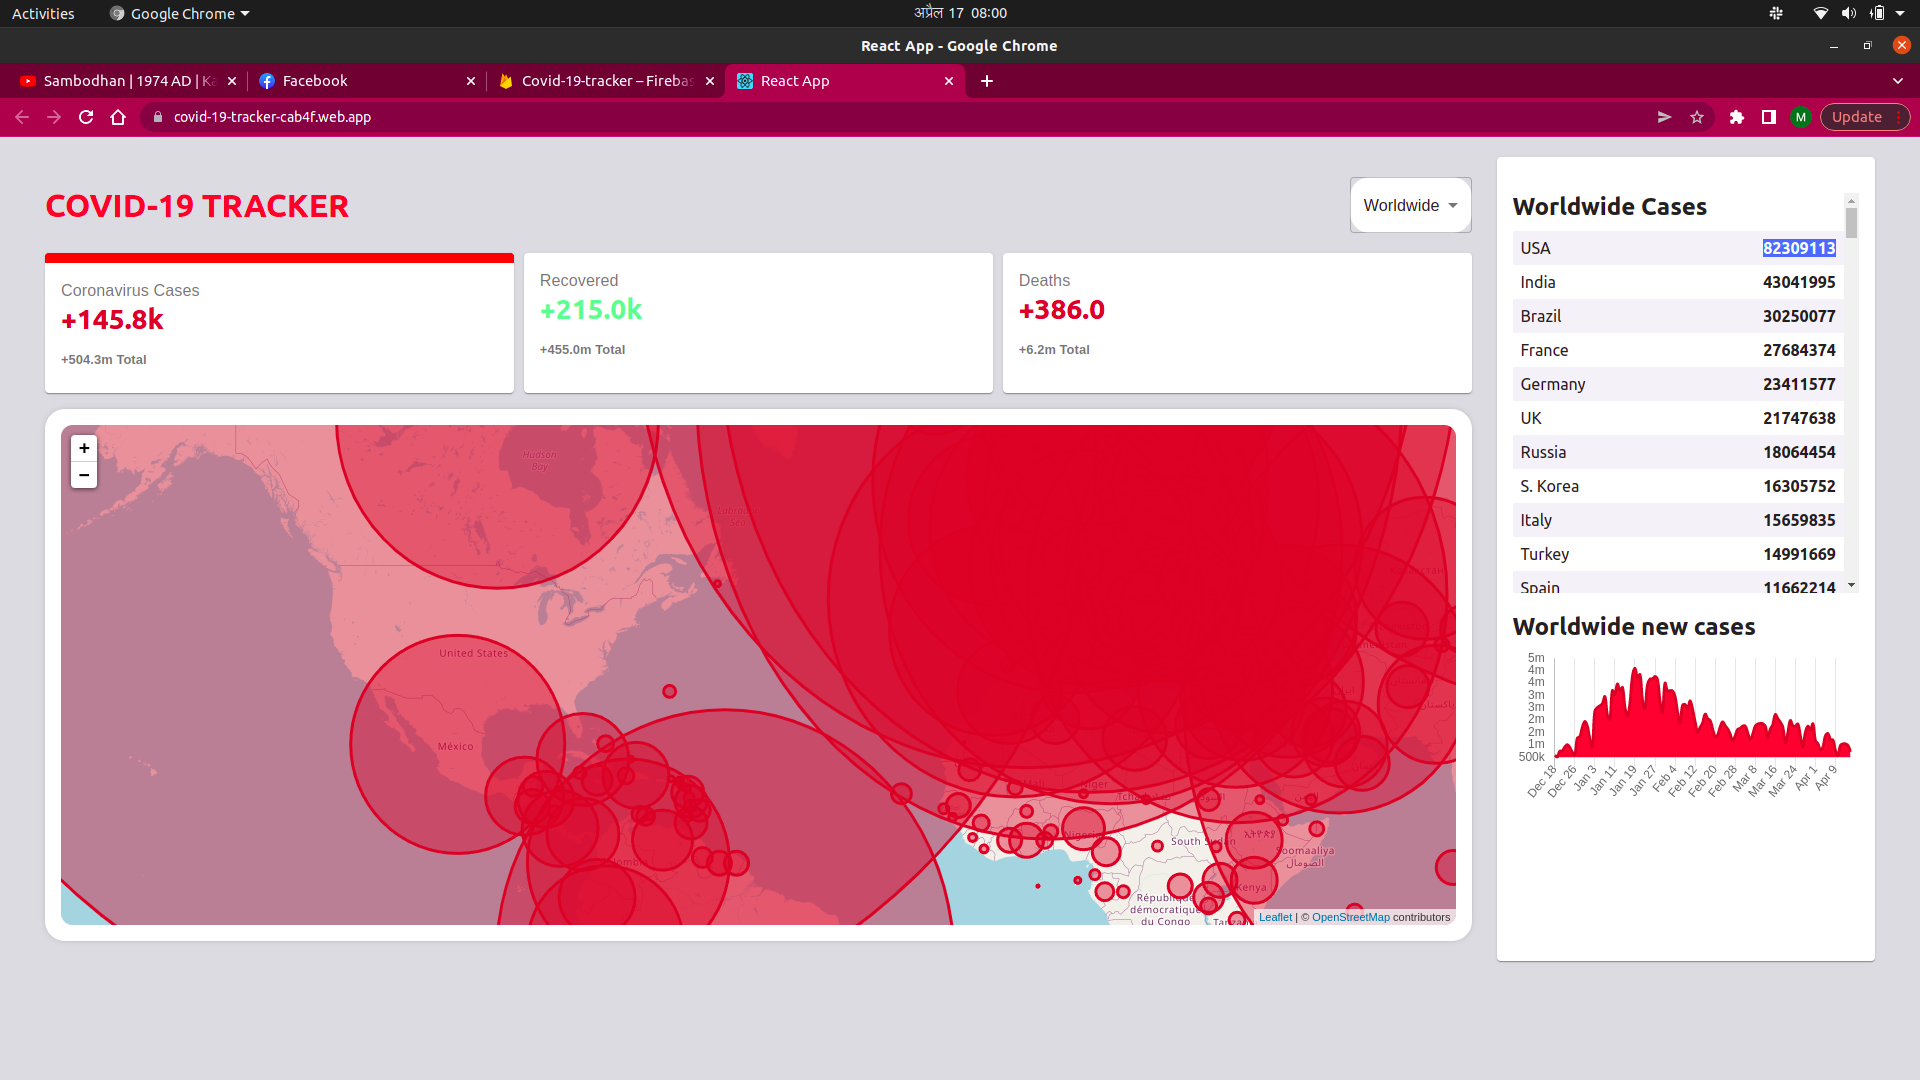
\includegraphics[scale=0.25]{data_covid.png}
   \caption{Recent Covid data(2022/4/17 6:34am)}
  \end{center}
  \end{figure}
  \pagebreak
  




\section{Overview}
The three basic important protocols to be followed are wearing mask, using hand sanitizer
or washing hand for at least up to 20 seconds, sanitizing own belongings which are used most
frequently. If there is any symptoms of fever and cough immediately take precaution and
isolate yourself from the crowd.
\\The primary purpose of this machine is that it can easily help us to follow above fundamental
protocols with in a one machine rather than having different system and places. The main
advantage of this machine is that we can check and sanitize with in one machine. The
machine works on power supply and also works on battery power.
\section{Background}
In this machine one can sanitize oneself and belongings intangibly, we use industrial grade
IR sensor in order to make the machine function intangibly. Also using Xray Images and CT scan images we are able to use 4 different transfer learning techniques to classify if Covid-19 is present or not.
\section{Problem Statement}
Realizing the effect of COVID-19 pandemic in the present scenario, a certain health protocol
has to be implemented in every human daily life routine. While going to some landmarks,
public places where a huge crowd is present, it is at owns sake to follow a certain protocol
to protect themselves from this dreadful virus. The pandemic has affected the whole world
mentally, physically as well as economically but this should not stop people from doing their
daily jobs. We can see security guards or some people holding a bottle of sanitizer and a
thermal gun to manually measure temperature and sanitize hand which is not feasible at
long term or at crowded places. Therefore, the machine we are proposing overcomes those
problem. In the context of Nepal, many mechanical innovations have been in use since
the pandemic to sanitize people in places like restaurant and landmark. The fault in those
products are they are tangible, but the machine we have proposed has tackled this issue as
it is intangible[2].

The most common COVID-19 detection technique is real-time polymerase chain
reaction (RT-PCR). It has a high percentage of false-negative findings and may take up
to two days to receive results, while having a sensitivity range of 70 to 90 \cite{ref9}; it may also
produce a quite high number of false-negative effects and may take up to two days to obtain
results. In some countries, it may take up to five days or more due to the overwhelming
number of tests that need to be analyzed \cite{ref4}.
Additionally, COVID-19 is detected and diagnosed using radiological screening tests
such as CXR and computed tomography (CT). 

It has been noticed that CXR is one of the
most effective methods for diagnosing pneumonia around the world because it is a rapid,
inexpensive, and popular clinical method that exposes the patient to less radiation than
CTs \cite{ref10,ref11}.
However, radiologists are needed to look for the radiological signs that show COVID19 symptoms on a CXR. To save time and effort, it is important to automate the CXR
analysis, which is a long and error-prone process that takes a lot of time and effort \cite{ref12}.

As a result, fully automated and real-time radiography image analyses are required
to assist physicians in accurately detecting COVID-19 infection. Physicians may use
computer-aided diagnosis (CAD) systems based on DL methods to help them perceive
and understand the information in CXR images as well as to overcome the limitations of
the imaging acquisition techniques used, rapidly and correctly. DL methods are becoming
more common in medical imaging because of their ability to deal with massive datasets
that surpass human capabilities. Combining CAD techniques with radiologist medical
diagnostics decreases physicians’ stress as well as improves their accuracy and statistical
analysis \cite{ref11}.
\section{Objectives}
The objectives of proposed project are given below:
\begin{itemize}
\item To prevent Covid-19 using X-ray and CT scan Images.
\item To predict Covid-19 Symptomps using patients datas.(Temperature, Oxygen Level, Pulse)
\item To prevent Covid-19 by following WHO protocols.

\end{itemize}
\section{Project Features}
The features of proposed projects are given below:
\begin{itemize}
\item Infrared thermometer to measure a person’s body temperature.
\item UV ray to sterilize the belongings
\item Proximity Sensor to function the process of sanitizing, sterilizing and measuring temperature intangibly.
\item The health monitoring system measures the vital criteria like temperature, Pulse, SPO2 and predicts COVID symptoms.
\item Covid Detection using CNN (VGGNet, ResNet, Inception, Xception)
\end{itemize}
\section{Feasibility}
Technically speaking this is crucial part of the system because it decides whether the concept
is achievable in real life or not. Most of the system analysis enhances the best utilization of
money, resources as well as time. So before carrying out detail system analysis, certain time
was devoted in dealing with feasibility study.
\subsection{Economical Feasibility}
This project is quite cost effective as the hardware components that we will be using in the
construction of this device are easily available in the market and are cheap apart from the
Infrared Thermal sensor. Since the temperature we need to measure should follow health
and medical standard we have reverse engineered Infrared Thermal Gun and made it work
automatically using proximity sensor. 
\subsection{Technical Feasibility}
Our project seems to be technically feasible on its structural development and its hardware
requirement, since it uses less number of sensors and other electronic components. By using
the limited numbers of sophisticated electronic components we can receive the desired output.
This project is based on modern technology based hardware components and devices which
will be very applicable in real life. We have selected the hardware components in such a
manner that this project is technically feasible.
\subsection{Operational Feasibility}
As this system is stationary with multiple functionality, it is every efficient because the
proximity sensor we are using is of industrial grade. The system works both on power supply
as well a 12 V lead acid battery. Also
this is a 4 in 1 machine that sanitizes, sterilizes and measures temperature
without even touching the machine.
\chapter{Literature Review}
COVID-19 (coronavirus disease 2019) is an infectious disease caused by severe acute respiratory syndrome coronavirus 2 (SARS-CoV-2), previously known as the 2019 novel coronavirus (2019-nCoV), a species of coronavirus. On 11 February 2020, the WHO officially renamed the clinical condition COVID-19.
Coronaviruses (CoV) are a large family of viruses that cause illness ranging from the common cold to more severe diseases such as Middle East Respiratory Syndrome (MERS-CoV) and Severe Acute Respiratory Syndrome (SARS-CoV). A novel coronavirus (nCoV) is a new strain that has not been previously identified in humans.
It is believed to have zoonotic origins and has close genetic similarity to bat coronaviruses, suggesting it emerged from a bat-borne virus
Infected patients show common signs include respiratory symptoms, fever, cough, shortness of breath and breathing difficulties. In more severe cases, the infection can cause pneumonia, severe acute respiratory syndrome, kidney failure, and even death.
Pneumonia is an acute respiratory infection that affects the lungs. It is a fatal illness in which the air sacs get filled with pus and other liquid.\cite{ref1} There are mainly two types of pneumonia: bacterial and viral. Generally, it is observed that bacterial pneumonia causes more acute symptoms. The most significant difference between bacterial and viral pneumonia is the treatment. Treatment of bacterial pneumonia is done using antibiotic therapy, while viral pneumonia will usually get better on its own\cite{ref2}. It is a prevalent disease all across the globe. Its principal cause includes a high level of pollution. Pneumonia is ranked eight in the list of the top 10 causes of death in the United States \cite{ref4}.
According to the WHO, “Every year, it kills an estimated 1.4 million children under the age of five years, accounting for 18\% of all deaths of children under five years old worldwide. Pneumonia affects children and families everywhere but is most prevalent in South Asia and sub-Saharan Africa. Children can be protected from pneumonia. It can be prevented with simple interventions and treated with low-cost, low-tech medication and care” \cite{ref2}. Therefore, there is an urgent need to do research and development on computer-aided diagnosis so that the pneumonia-related mortality, especially in children, can be reduced.
One of the following tests can be done for pneumonia diagnosis: chest X-rays, CT of the lungs, ultrasound of the chest, needle biopsy of the lung, and MRI of the chest \cite{ref3}. Currently, chest X-rays are one of the best methods for the detection of pneumonia \cite{ref6}. X-ray imaging is preferred over CT imaging because CT imaging typically takes considerably more time than X-ray imaging, and sufficient high-quality CT scanners may not be available in many underdeveloped regions. In contrast, X-rays are the most common and widely available diagnostic imaging technique, playing a crucial role in clinical care and epidemiological studies \cite{ref5}.

Another issue with this disease is that sometimes, the features that describe the very existence of the disease often get mixed with other diseases, and hence, radiologists find it challenging to diagnose this disease. Deep learning techniques solve all these problems, and their accuracy in the prediction of the disease is the same and sometimes even greater than an average radiologist \cite{ref}. Among the deep learning techniques, convolutional neural networks (CNNs) have shown great promise in image classification and segmentation and therefore are widely adopted by the research community. Biomedical image diagnosis that uses the techniques of deep learning and computer vision has proven to be very helpful to provide a quick and accurate diagnosis of the disease that matches the accuracy of a reliable radiologist. Currently, deep learning based methods cannot replace trained clinicians in medical diagnosis, and they aim to supplement clinical decision making.

\section{Related Works}
This section provided an overview of some related studies for a better understanding
of the area under study and to provide the state-of-the-art picture. Convolutional neural
networks (CNNs), which are one of the most effective DL models, have successfully proved
their mastery over conventional methods in several disciplines, including image classification and pattern recognition \cite{ref13,ref14}. Currently, it has indeed been successfully implemented
in the field of medicine with impressive outcomes and outstanding performance in different
challenging settings. Various medical imaging systems using DL techniques have also been
developed to assist physicians and specialists in effective COVID-19 diagnosis, care, and
follow-up examination \cite{ref15,ref16}. Narin et al. \cite{ref11} used five-fold cross validation to enforce
various binary classifications. With an accuracy equal to 98per cent, specificity value of 100per cent,
and a recall with 96per cent, the pre-trained ResNet-50 method gives the best efficiency. On the
other hand, Wang et al. \cite{ref17} have suggested using CXR images to automatically establish a
new deep architecture called COVID-Net to detect COVID-19 instances. Using a database
containing 13,975 CXR images, this model has the highest classification accuracy of 93.3per cent.
The key strength of this approach is that the conceptual composition could create a balance
between different goals such as accuracy and computational costs through architectural
design choices.\\

Hemdan et al. \cite{ref18} introduced COVIDXNet, a DL framework for detecting
COVID-19 infections in CXR images. A small dataset of 50 images was used to compare
seven DL techniques (e.g., MobileNetV2, ResNetV2, VGG19, DenseNet201, InceptionV3,
Inception, and Xception). DenseNet201 had the best performance, with a 91per cent accuracy
score. While Zhang et al. \cite{ref19} derived useful feature representations from CXR image
using ResNet-18 model as a feature vector. Those derived features were then entered as
an input into a multi-layer perception. A dataset of hundred images taken from seventy
patients yielded the highest accuracy rate of 96per cent. A further supervised transfer-learning
method for COVID-19 infection detection in CXR using an extreme version of the Xception
model was developed by Das et al. \cite{ref12}, which achieved accuracy of 97.4per cent. Furthermore,
Ozturk et al. \cite{ref20} introduced a new system for COVID-19 identification using CXR for
automatic detection. It was created to provide consistent and reliable diagnostics for
multi-class classifications (COVID-19, mild, and pneumonia) and binary classifications
(COVID vs. non-COVID). Using the DarkNet model, they were able to achieve a classification performance of 98.08per cent for binary classification and 87.02per cent for the classification
of multi-class.
Many studies have tried to find COVID-19 infections in CXR images by using different
DL methods. The investigation of COVID-19 identification
and diagnostic systems that rely on CXR images indicated that there are still a number
of vulnerabilities that need additional investigation. For starters, the majority of current
systems have been validated with limited CXR datasets as well as a small presence of
positive COVID-19 cases. The size of the datasets is insufficient to indicate the true output
of the proposed systems. Furthermore, despite the fact that several researchers have
achieved high reliability values using pre-trained models through transfer-learning, there
has been little focus on developing and training a customized DL model from scratch due
to a shortage of a large dataset including a substantial number of CXR images with reported
COVID-19 infection.




\section{ Sanitizing Machine in Market}
\subsection{ Fogger Machine}
Figure 2.1 shows the fogger machine. This fogger machine produces special fog to the surrounding which kills the viruses present in the air as well as surfaces.
 \begin{figure}[h]  % h means here
   \begin{center}
   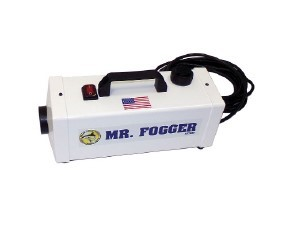
\includegraphics[scale=0.7]{fogger.jpg}
   \caption{Fogger Machine}
  \end{center}
  \end{figure}
\subsection{ UV sterilizing Machine}
Figure 2.2 shows the fogger machine. This fog machine produces special fog to the surrounding which kills the viruses present in the air as well as surfaces.
 \begin{figure}[h]  % h means here
   \begin{center}
   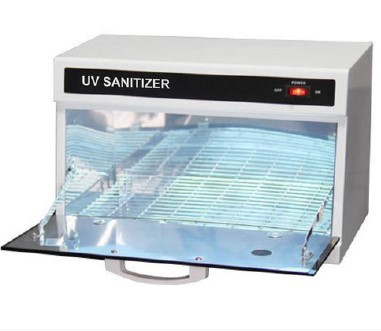
\includegraphics[scale=0.7]{uv machine.jpg}
   \caption{UV Sterilizing Machine}
   \end{center}
  \end{figure}
\chapter{System Requirement}
\section{Software Requirement}
\subsection{Python IDE}
Python is an interpreted high-level general-purpose programming language. Python’s design
philosophy emphasizes code readability with its notable use of significant indentation. Its
language constructs as well as its object-oriented approach aim to help programmers write
clear, logical code for small and large-scale projects. We use python in order to perform
machine learning to predict the symptoms of COVID with higher accuracy
\subsection{Arduino IDE}
The Arduino Software (IDE) includes a text editor for writing code, a message area, a text
console, a toolbar with buttons for basic functions, and a series of menus. It communicates
with the Arduino and Genuino devices by connecting to them and uploading code. Sketches
8 are programs created with the Arduino Software (IDE). These sketches were created with
7
a text editor and saved with the.ino file extension. The message section indicates faults and
provides feedback while storing and exporting. The Arduino Software (IDE) outputs text
to the console, which includes detailed error messages and other information.
\pagebreak
\section{Hardware Requirement}
\subsection{Arduino}
Arduino is an open-source electronics platform based on easy-to-use hardware and software.
Arduino boards are able to read inputs - light on a sensor, a finger on a button, or a Twitter
message - and turn it into an output - activating a motor, turning on an LED, publishing
something online. It can tell your board what to do by sending a set of instructions to the
microcontroller on the board.
\begin{figure}[h] % h means here
   \begin{center}
   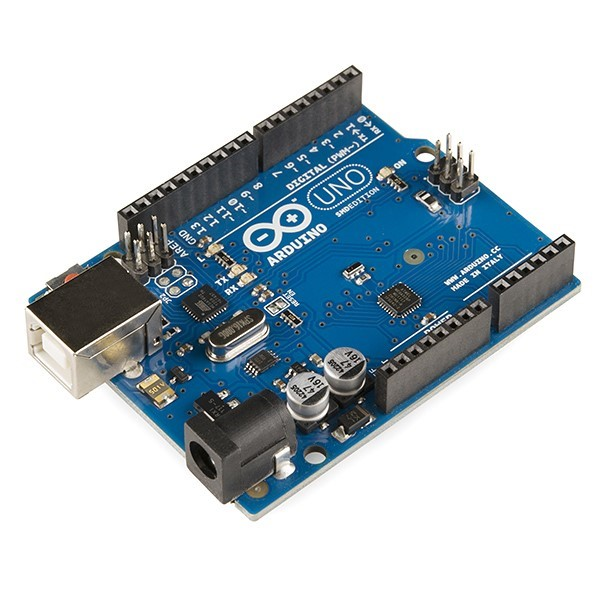
\includegraphics[scale=0.8]{arduino.jpg}
   \caption{Arduino}
  \end{center}
  \end{figure}
\subsection{Infrared Thermometer}
This is the equipment used to measure the temperature of the human body without touching
surface.
\begin{figure}[h] % h means here
   \begin{center}
   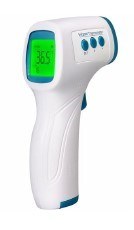
\includegraphics[scale=0.6]{ir thermo.jpg}
   \caption{IR Thermometer}
  \end{center}
  \end{figure}
  \pagebreak
\subsection{Car Wiper Motor}
The car wiper motor is the component that powers the windshield wipers. As it spins, a
mechanism built to it rotates a worm gear, arm and, finally, the windshield or windscreen
wiper blades. The wiper blades then rid the windscreen of water, snow, dust, or any other
debris that may affect visibility when driving.
\begin{figure}[h] % h means here
   \begin{center}
   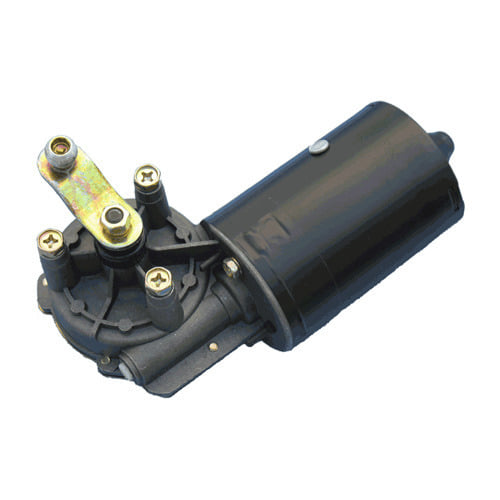
\includegraphics[scale=0.3]{car.jpg}
   \caption{Car Wiper Motor}
  \end{center}
  \end{figure}
\subsection{Raspberry Pi}
The Raspberry Pi is a low cost, credit-card sized computer that plugs into a computer
monitor or TV, and uses a standard keyboard and mouse. It is a capable little device that
enables people of all ages to explore computing, and to learn how to program in languages
like Scratch and Python.The original Pi had a single-core 700MHz CPU and just 256MB
RAM, and the latest model has a quad-core CPU clocking in at over 1.5GHz, and 4GB
RAM.
\begin{figure}[h] % h means here
   \begin{center}
   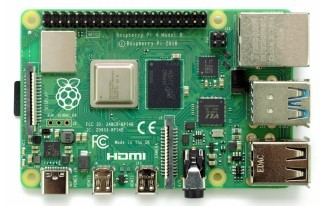
\includegraphics[scale=1]{rb pi.jpg}
   \caption{Raspberry Pi}
  \end{center}
  \end{figure}
\pagebreak
\subsection{IR proximity sensor:}
Proximity Sensor are used to detect objects and obstacles in front of sensor. Sensor keeps
transmitting infrared light and when any object comes near, it is detected by the sensor by
monitoring the reflected light from the object
\begin{figure}[h] % h means here
   \begin{center}
   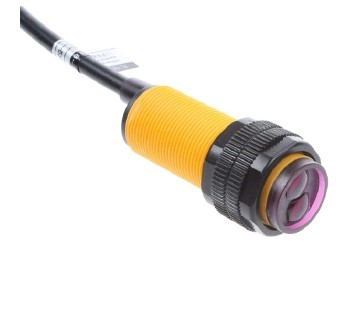
\includegraphics[scale=0.5]{ir sensor.jpg}
   \caption{IR Proximity Sensor}
  \end{center}
  \end{figure}

\subsection{MAX30100}
The MAX30100 is a sensor that combines pulse oximetry and a heart rate monitor. It
detects pulse oximetry and heart rate signals using two LEDs, a photo detector, improved
optics, and low-noise analog signal processing. It’s an optical sensor that derives its readings
from emitting two wavelengths of light from two LEDs – a red and an infrared one – then
measuring the absorbance of pulsing blood through a photo detector. This particular LED
colour combination is optimized for reading the data through the tip of one’s finger.
 \begin{figure}[h] % h means here
   \begin{center}
   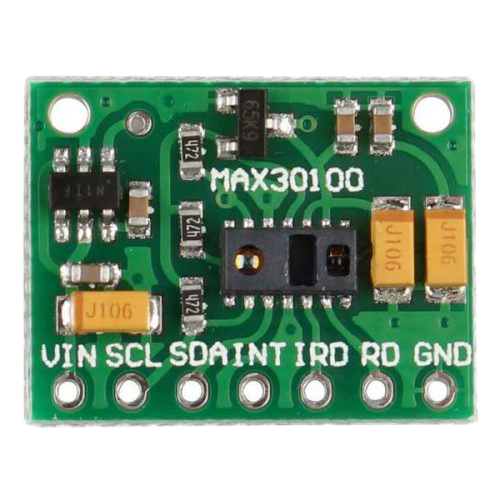
\includegraphics[scale=0.3]{oxi.png}
   \caption{Oxymeter}
  \end{center}
  \end{figure}
  \
\subsection{ Pump Motor}
Pump is a mechanical device that converts mechanical torque into hydraulic energy. It
simply facilitates movement of fluids from one place to another using suction or pressure or both. Motors, on the other hand, are electro-mechanical devices that are used to convert
electrical energy into mechanical energy.
\begin{figure}[h] % h means here
   \begin{center}
   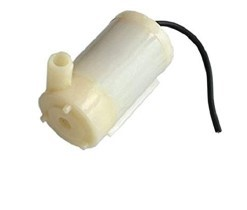
\includegraphics[scale=0.5]{pump motor.jpg}
   \caption{Pump Motor}
  \end{center}
  \end{figure}
\subsection{Temperature Sensor}
The MAX30205 temperature sensor accurately measures temperature and provide an over
temperature alarm/interrupt/shutdown output. This device converts the temperature measurements to digital form using a high resolution, sigma-delta, analog-to-digital converter
(ADC).
\begin{figure}[h] % h means here
   \begin{center}
   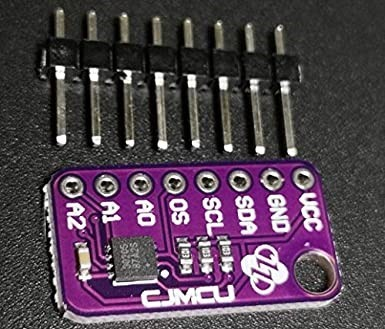
\includegraphics[scale=0.7]{temp sensor.jpg}
   \caption{Temperature Sensor}
  \end{center}
  \end{figure}
  \
\subsection{UV-C Tube Light}
With a 99.9 effective rate, UVC LED Tubes can kill viruses promptly. Viruses are known
for lingering on surfaces for a few hours to several days at a time. It is extremely sensitive
to ultraviolet light and scientists have confirmed that the virus can be killed at certain
exposures of UV.
\begin{figure}[h] % h means here
   \begin{center}
   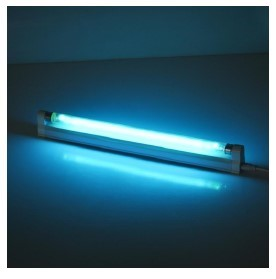
\includegraphics[scale=0.6]{uv c.jpg}
   \caption{UV-C Tube Light}
  \end{center}
  \end{figure}
\chapter{Methodology}
This project includes four major parts, which are mainly used in COVID-19 safety protocols.
Mask detection part detects mask on the face of the people, automatic temperature portion
takes reading of the temperature of wrist of the people and shows on the display temperature
reading in the LCD screen. To maintain the medical standard, we have reversed engineered
the medical infrared thermal gun for this project. As we know most of the viruses transfer
through hand and it has to be sanitize regularly so automatic hand sanitizer helps to sanitize
our hand without touching any surfaces.

Finally, we have UV-C chamber in this project which is used to disinfect the person’s belongings like bag, cloths, documents and cash etc. many of the research verified that exposer
of viruses in UV-C kills the viruses more easily. Many country are also using 
UV-C to kill pathogens or to disinfect the tools and other things.\\
The flow chart and block diagram of working are described below:
\section{Block Diagram of Covid Prevention}
\subsection{Temperature Sensor}
In this project, the reversed engineered Thermal Gun will measure human body temperature
sensor will be interface to reach the health and safety standard and display it digitally.
\begin{figure}[h] % h means hereRGB 
   \begin{center}
   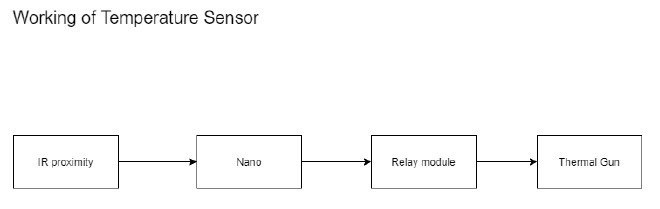
\includegraphics[scale=0.8]{medical ventilation.jpg}
  \end{center}
  \end{figure}
  \pagebreak
\subsection{Sanitizer Dispenser}
In this project, a proximity sensor is used to turn on relay module which will turn on pump moter and sanitizer will be dispensed.
\begin{figure}[h] % h means here
   \begin{center}
   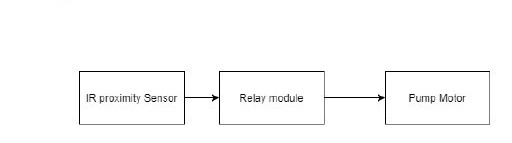
\includegraphics[scale=0.8]{block diagram u v c.jpg}
  \end{center}
  \end{figure}
  \section{Block Diagram of Covid Detection}
  \subsection{Detection using Clinical datas}
  \subsubsection{Collection of Clinical Datas}
  First we collected clinical datas like Age,Temperature,Oxygen percentage,pulse reading and heart beat.
  \begin{figure}[h] % h means here
   \begin{center}
   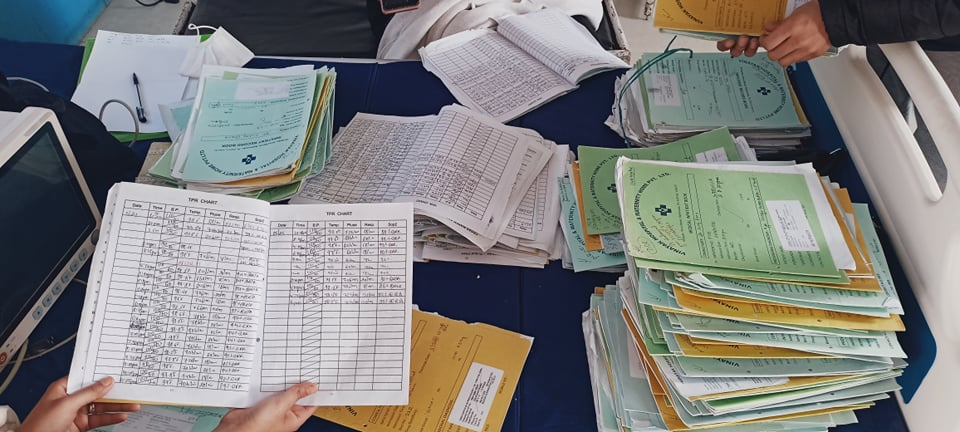
\includegraphics[scale=0.3]{collection.jpg}
   \caption{Data Collection Process}
  \end{center}
  \end{figure}

  \subsubsection{Entry of Clinical Datas}
  After collecting the data we have prepared it in digital format. This process also got rid of empty data and data preprocessing process.We collected a total of 150 data from differene patients.This will now be used to implement our model.
  \begin{figure}[h] % h means here
   \begin{center}
   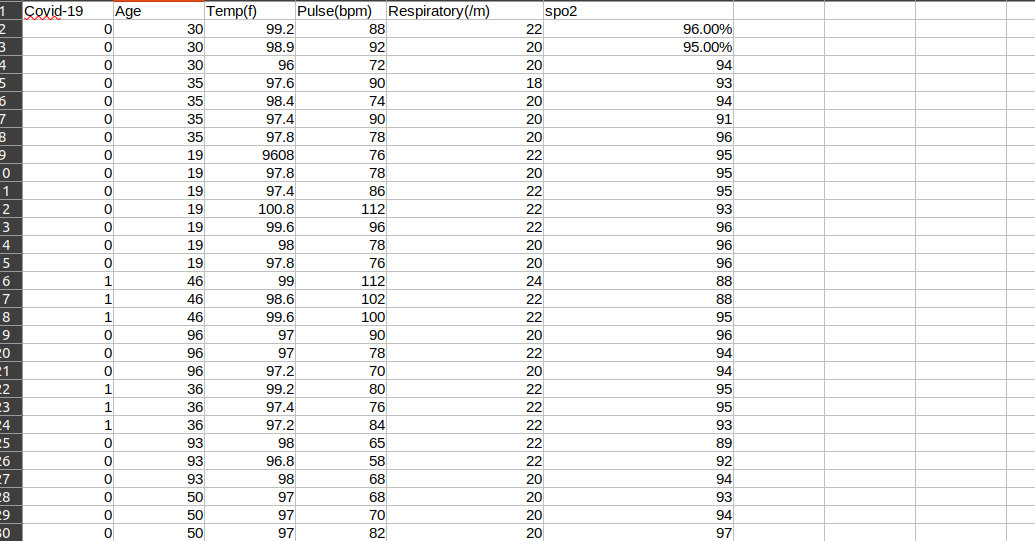
\includegraphics[scale=0.4]{excel.png}
   \caption{Data Collection Process}
  \end{center}
  \end{figure}
\subsubsection{Logistic Regression}
Logistic regression is a process of modeling the probability of a discrete outcome given an
input variable. The most common logistic regression models a binary outcome; something
that can take two values such as true/false, yes/no, and so on. Multinomial logistic regression can model scenarios where there are more than two possible discrete outcomes. Logistic
regression is a useful analysis method for classification problems, where you are trying to
determine if a new sample fits best into a category. As aspects of cyber security are classification problems, such as attack detection, logistic regression is a useful analytic technique.
\begin{figure}[h] % h means here
   \begin{center}
   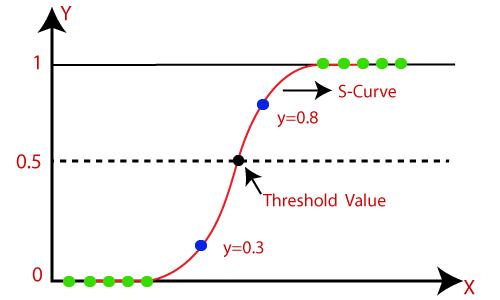
\includegraphics[scale=0.6]{regression.png}
   \caption{Logistic Regression}
  \end{center}
  \end{figure}

  \begin{figure}[h] % h means here
   \begin{center}
   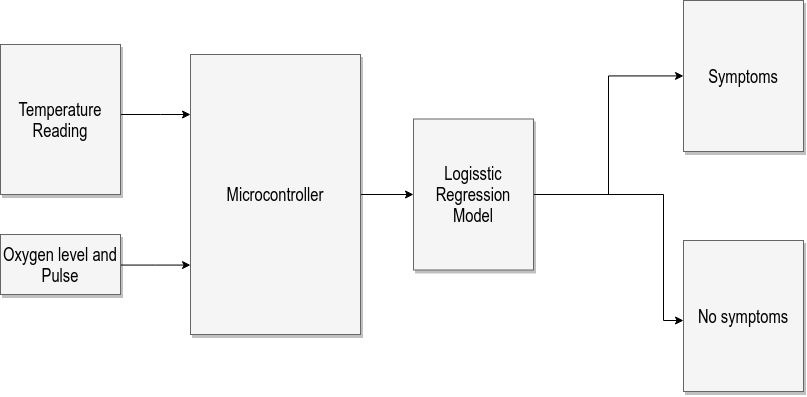
\includegraphics[scale=0.6]{logistic.png}
   \caption{Logistic regression}
  \end{center}
  \end{figure}
  
  \pagebreak
    \subsection{Detection using Xray Images}
\subsubsection{Colletion of Xray data}
First we collected chest Xray images from Sumeru City Hospital which was already labeled as covid or normal.
\begin{figure}[h] % h means here
   \begin{center}
   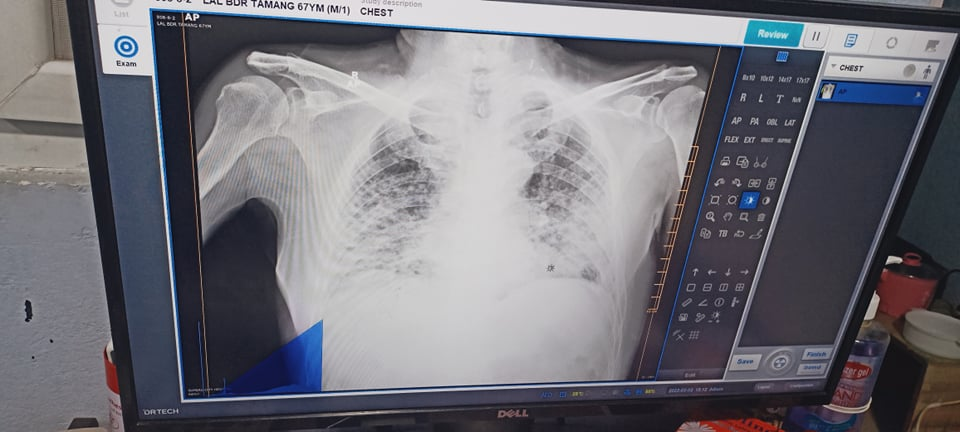
\includegraphics[scale=0.2]{xray1.jpg}
   \caption{Xray of Covid Patient}
  \end{center}
  \end{figure}
  \begin{figure}[h] % h means here
   \begin{center}
   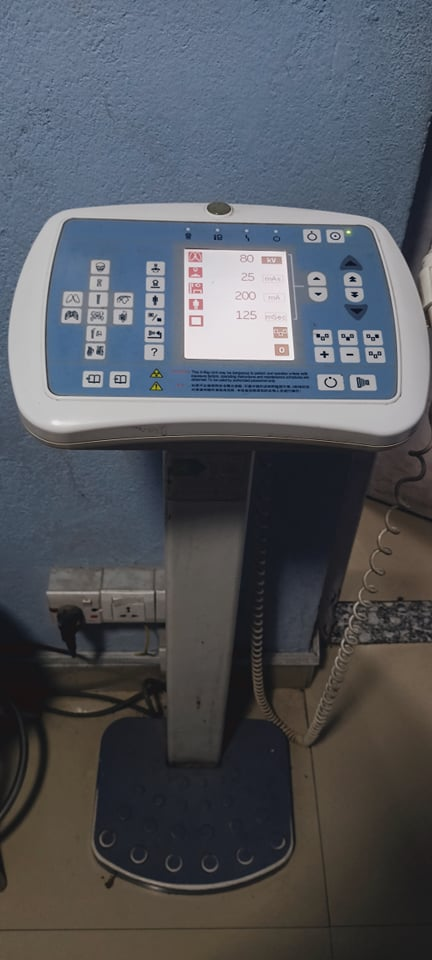
\includegraphics[scale=0.2]{xray2.jpg}
   \caption{Xray machine Controller}
  \end{center}
  \end{figure}
  \pagebreak
\subsubsection{Convolutional Neural Networks}
A Convolutional Neural Network (ConvNet/CNN) is a Deep Learning algorithm which can
take in an input image, assign importance (learnable weights and biases) to various aspects/objects in the image and be able to differentiate one from the other. The pre-processing
required in a ConvNet is much lower as compared to other classification algorithms. While
in primitive methods filters are hand-engineered, with enough training, ConvNets have the
ability to learn these filters/characteristics.
\\
CNN develops an automatic diagnostic system which uses chest X-ray analysis results to diagnose whether a person is COVID-19-affected or normal. The study begins with collection of primary dataset containing two image classes: one class belonged to chest X-rays of COVID-19-confirmed cases and the other class of images belonged to the normal people without the disease. The open source dataset is concerned medical professionals analysed the dataset and removed some of the X-ray images which were not clear in terms of quality and diagnostic parameters which result dataset very clean, as each X-ray image was of good quality as well as clear in terms of significant diagnostic parameters according to their expertise.The dataset will be augmented to increase its size. The resulted dataset is used to train the model in the next phase. After training, the model will be tested for its performance in the disease detection. The testing of proposed CNN model has been done using test dataset held from the primary dataset as well as using the independent validation dataset.
\begin{figure}[h] % h means here
   \begin{center}
   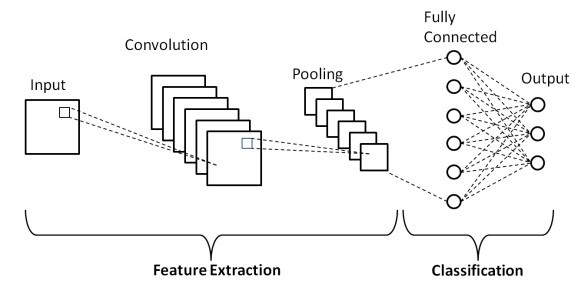
\includegraphics[scale=0.8]{cnn.jpg}
   \caption{Convolutional Neural Network}
  \end{center}
  \end{figure}
\subsubsection{VGGNet-16}
The full name of VGG is the Visual Geometry Group.It has released a series of convolutional network models beginning with VGG, which can be applied to face recognition and image classification, from VGG16 to VGG19. The original purpose of VGG's research on the depth of convolutional networks is to understand how the depth of convolutional networks affects the accuracy and accuracy of large-scale image classification and recognition. -Deep-16 CNN), in order to deepen the number of network layers and to avoid too many parameters, a small 3x3 convolution kernel is used in all layers.

The input of VGG is set to an RGB image of 224x244 size. The average RGB value is calculated for all images on the training set image, and then the image is input as an input to the VGG convolution network. A 3x3 or 1x1 filter is used, and the convolution step is fixed. . There are 3 VGG fully connected layers, which can vary from VGG11 to VGG19 according to the total number of convolutional layers + fully connected layers. The minimum VGG11 has 8 convolutional layers and 3 fully connected layers. The maximum VGG19 has 16 convolutional layers. +3 fully connected layers. In addition, the VGG network is not followed by a pooling layer behind each convolutional layer, or a total of 5 pooling layers distributed under different convolutional layers. The following figure is VGG Structure diagram:

  \begin{figure}[h] % h means here
   \begin{center}
   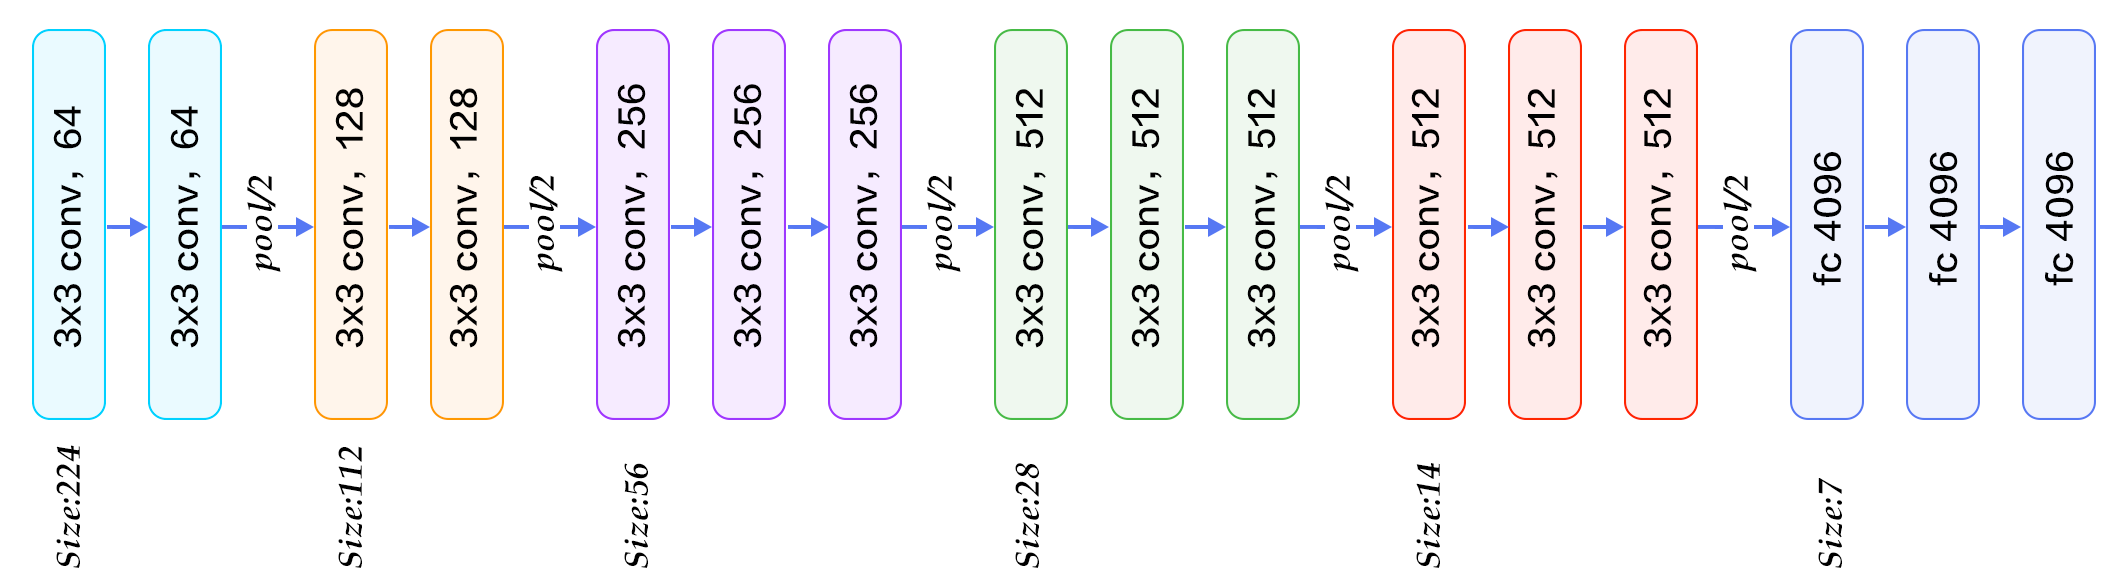
\includegraphics[scale=0.2]{vgg.png}
   \caption{VGG architecture}
  \end{center}
  \end{figure}
  
  \begin{figure}[h] % h means here
   \begin{center}
   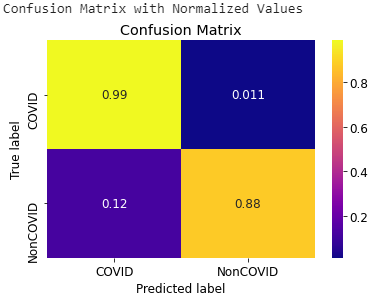
\includegraphics[scale=0.6]{vgg_chest_cm.png}
   \caption{VGG Confusion Matrix}
  \end{center}
  \end{figure}
\subsubsection{ResNet50}
ResNet-50 is a convolutional neural network that is 50 layers deep. You can load a pretrained version of the network trained on more than a million images from the ImageNet database. The pretrained network can classify images into 1000 object categories, such as keyboard, mouse, pencil, and many animals. Unlike traditional sequential network architectures such as AlexNet, OverFeat, and VGG, ResNet is instead a form of “exotic architecture” that relies on micro-architecture modules.
\begin{figure}[h] % h means here
   \begin{center}
   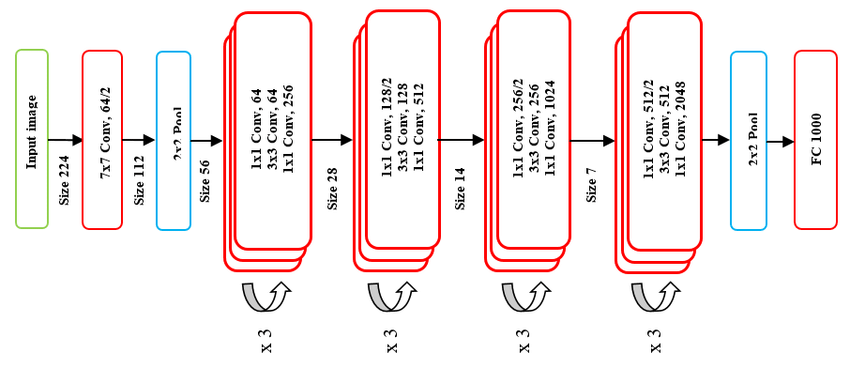
\includegraphics[scale=0.4]{resnet.png}
   \caption{Resnet}
  \end{center}
  \end{figure}

  \begin{figure}[h] % h means here
   \begin{center}
   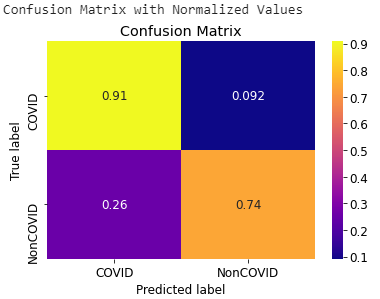
\includegraphics[scale=0.6]{resnet_chest_cm.png}
   \caption{Resnet Confusion Matrix}
  \end{center}
  \end{figure}
    \pagebreak
  \subsubsection{Inception-V3}
Inception-V3 is a convolutional neural network that is 48 layers deep. You can load a pretrained version of the network trained on more than a million images from the ImageNet database. The pretrained network can classify images into 1000 object categories, such as keyboard, mouse, pencil, and many animals. As a result, the network has learned rich feature representations for a wide range of images. The network has an image input size of 299-by-299.
\begin{figure}[h] % h means here
   \begin{center}
   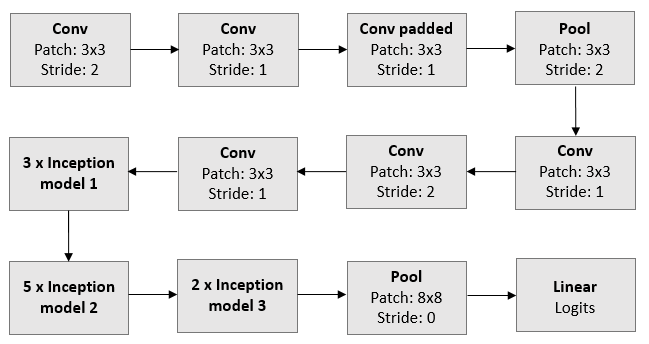
\includegraphics[scale=0.5]{inception.png}
   \caption{Inception-V3}
  \end{center}
  \end{figure}

  \begin{figure}[h] % h means here
   \begin{center}
   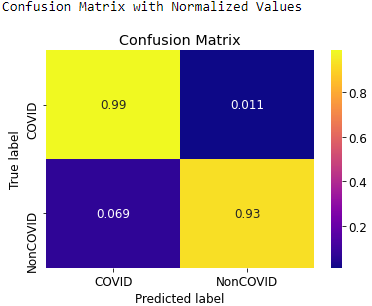
\includegraphics[scale=0.6]{inception_chest_cm.png}
   \caption{Inception Confusion Matrix}
  \end{center}
  \end{figure}
  
  \pagebreak
  
  \subsubsection{Xception}
Xception is a convolutional neural network that is 71 layers deep. You can load a pretrained version of the network trained on more than a million images from the ImageNet database. The pretrained network can classify images into 1000 object categories, such as keyboard, mouse, pencil, and many animals. As a result, the network has learned rich feature representations for a wide range of images. The network has an image input size of 299-by-299.
\begin{figure}[h] % h means here
   \begin{center}
   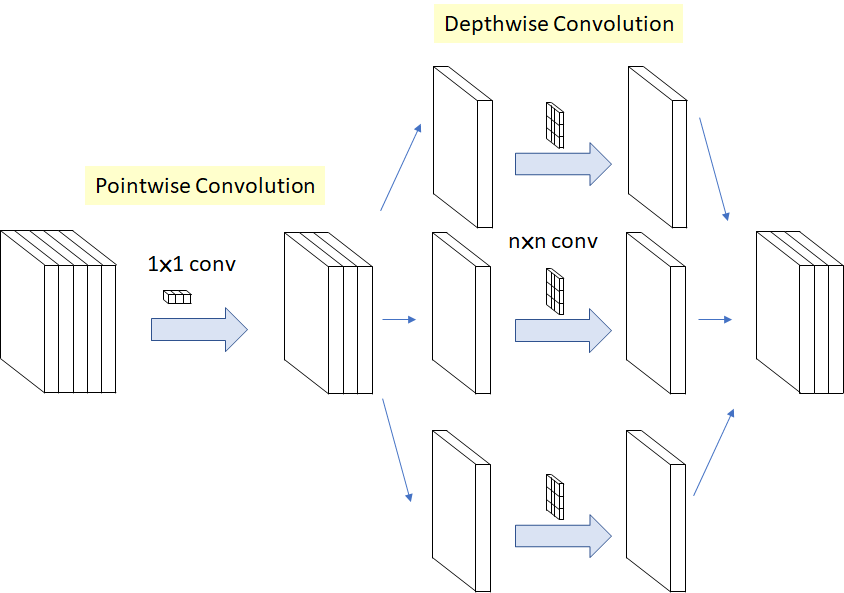
\includegraphics[scale=0.4]{xception.png}
   \caption{Xception}
  \end{center}
  \end{figure}
  \begin{figure}[h] % h means here
   \begin{center}
   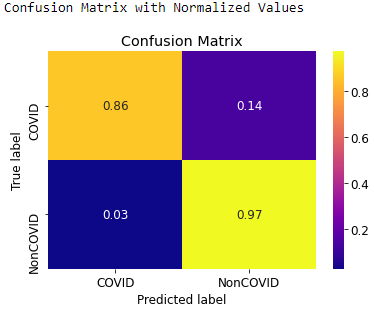
\includegraphics[scale=0.8]{xception_chest_cm.png}
   \caption{xception Confusion Matrix}
  \end{center}
  \end{figure}



\pagebreak
\chapter{Epilogue}
\section{Expected Outcome}
The following mentioned outcomes or results are highly expected:

\begin{itemize}
\item Semi tangible machine
\item Measures human temperature, oxygen saturation level and heart beat rate and analyzes
them to assure COVID symptoms
\item Show recent Covid datas and news.
\item Analyse X Ray and CT scan images for Covid-19 detection.
\end{itemize}
\section{Application}
\begin{itemize}
\item To measure human temperature, oxygen saturation level and heart beat rate.
\item To compare the data and analyse whether people carry COVID symptoms or not.
\item To disinfect cash in banks, medical or surgical tools in hospitals and others.
\item To analyze X Ray and CT scan images for Covid-19 detection. 
\end{itemize}
\pagebreak
\section{Budget Analysis}
\begin{table}[h]%h refers for here 
\centering
\begin{tabular}{|c|c|c|c|c|}
	
	\hline
	\textbf{SN} & \textbf{Hardware Required} & \textbf{Quantity} & \textbf{Unit Price} &\textbf{ Total}\\
	\hline
	1 & Arduino & 1 & 900 & 900 \\
	\hline
	2 & IR Proximity Sensor & 2 & 1000 & 2000\\
	\hline
	3 & Indicator & 3 & 20 & 60\\
	\hline
	4 & Power Switch  & 4 & 15 & 60\\
	\hline
	5 & 4 Channel Relay Module & 1 & 250 & 250 \\
  \hline
  6 & Rasberry Pi & 1 & 5000 & 5000 \\
  \hline
  7 & Pump Motor & 1 & 150 & 150 \\
  \hline
  8 & Power Window Motor & 1 & 1200 & 1200 \\
  \hline
  9 & USB Camera & 1 & 300 & 300 \\
  \hline
  10 & Lead Acid Battery & 1 & 1000 & 1000 \\
  \hline
   11 & Temperature Sensor (max 30205) & 1 & 1200 & 1200\\
\hline
   12 & Sp$O_2$ Sensor(max  30100) & 1 & 1600 & 1600\\
\hline
   13 & Infrared Thermometer & 1 & 2000 & 2000\\
\hline
 14 & IR Sensor & 1 & 100 & 100 \\
  \hline
Total: &  &  &  & 15820 \\
\hline
\end{tabular}
\caption{Budget Analysis }
\label{aaa}

\end{table}
\section{Work Schedule}
 The work schedule followed for various parts of our project is shown in following chart:\\ \\
 \begin{figure}[h]  % h means here
   \begin{center}
   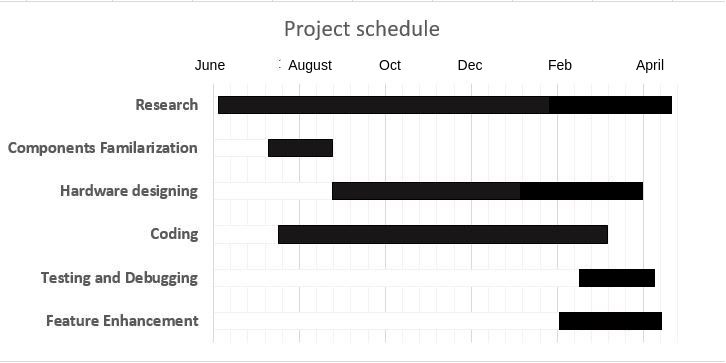
\includegraphics[scale=0.5]{gantt.jpg}
   \caption{Gantt Chart}
  \end{center}
  \end{figure}
  \pagebreak
  \subsection{Work Completed}
  \begin{itemize}
\item Analysed and Checked Covid Prevention Machine.
\item Obtained Xray and CT Scan Images dataset from Kaggle and Sumeru City Hospital.
\item Created a Model and Web Application of Covid Detection.
\item Created a Web application to show recent Covid-19 Statistics.
\item Obtained dataset of clinical data from different patients from Binayak Hospital and digitalized the data.
\item Created Web Application to predict Covid Symptoms
\end{itemize}

\begin{figure}[h]  % h means here
   \begin{center}
   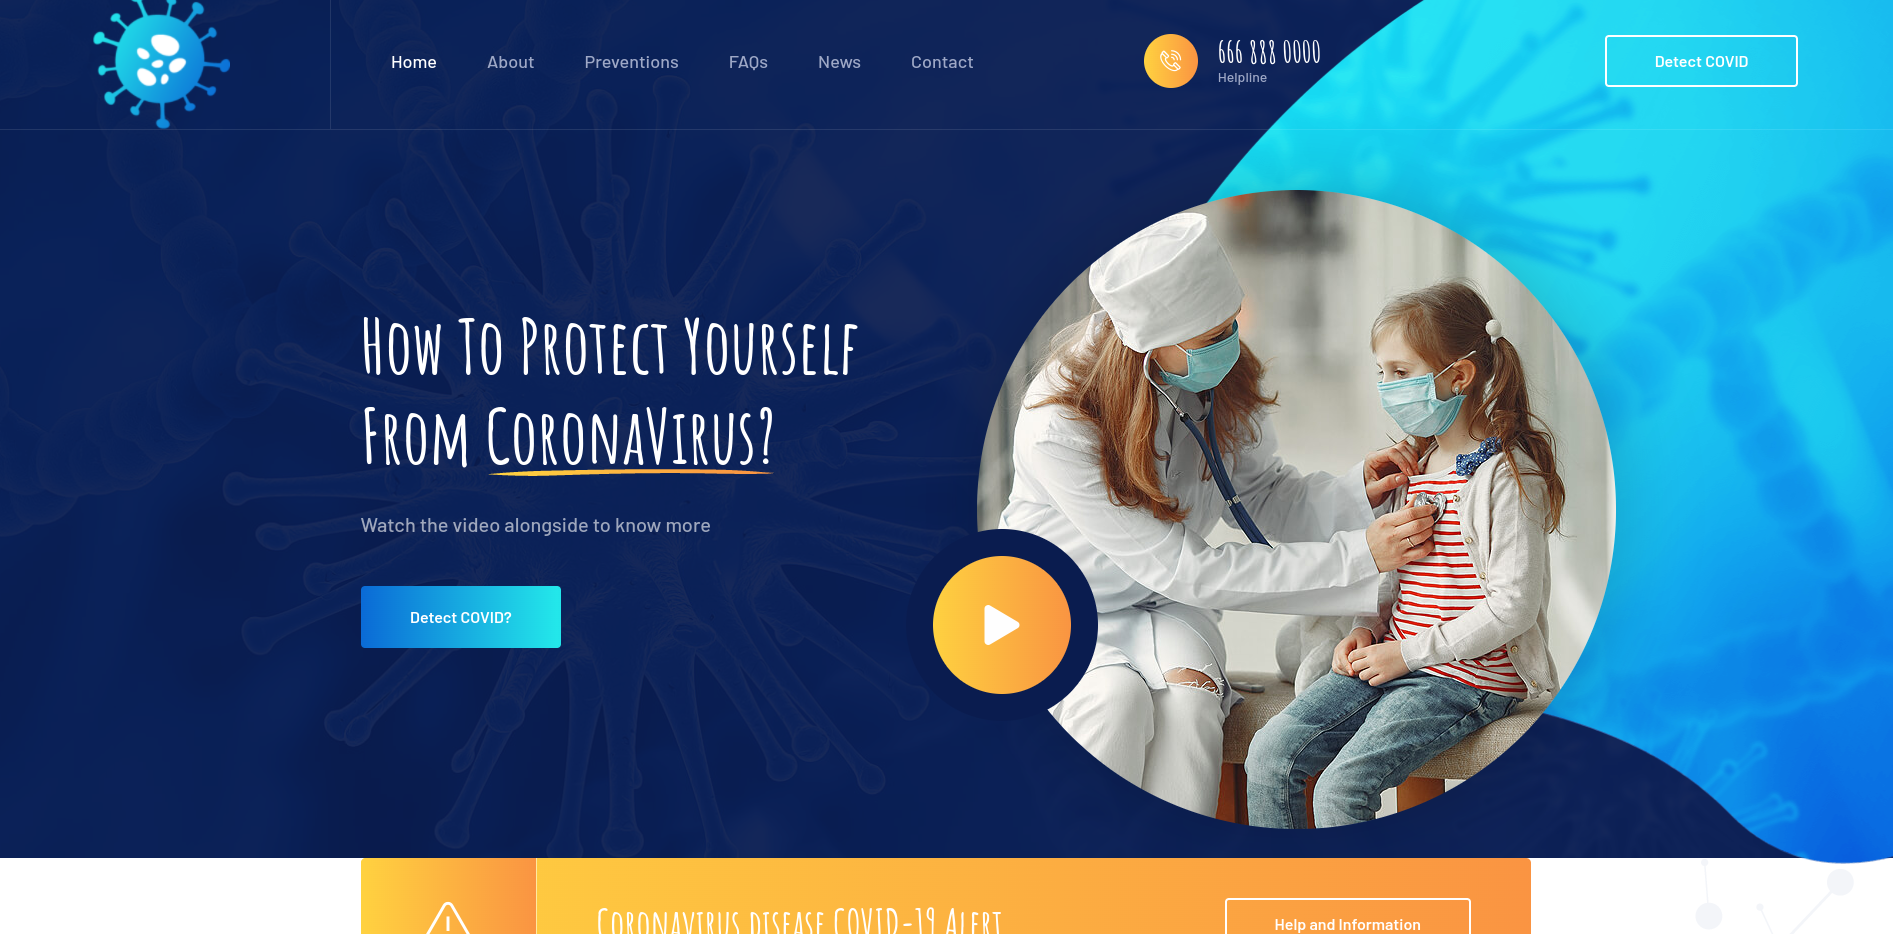
\includegraphics[scale=0.2]{detect.png}
   \caption{Covid Detection Web Application}
  \end{center}
  \end{figure}
\subsection{Work Remaining}
  \begin{itemize}
\item Implementing Raspberry pi to send data to database.
\end{itemize}
  \pagebreak
\addcontentsline{toc}{chapter}{Bibliography}
\bibliographystyle{plain}
\bibliography{references}
\end{document}
